\documentclass[20pt,margin=1in,innermargin=-4.5in,blockverticalspace=-0.25in]{tikzposter}
\geometry{paperwidth=42in,paperheight=30in}
\usepackage[utf8]{inputenc}
\usepackage{amsmath}
\usepackage{amsfonts}
\usepackage{amsthm}
\usepackage{amssymb}
\usepackage{mathrsfs}
\usepackage{graphicx}
\usepackage{adjustbox}
\usepackage{enumitem}
\usepackage[backend=biber,style=numeric]{biblatex}
\usepackage{emory-theme}

\usepackage{mwe} % for placeholder images
\usepackage{hyperref}
\usepackage{caption}
\usepackage{subcaption}
\usepackage{diagbox}
\graphicspath{ {./images/} }

% set theme parameters
\tikzposterlatexaffectionproofoff
\usetheme{EmoryTheme}


\title{A Hierarchical Structured Self-Attentive Model for Extractive Document Summarization}
\author{Koren Maliniak (ID. 200319572)
Or Stern (ID. 305698664)}
\institute{IDC, Israel}

% begin document
\begin{document}
\maketitle
\centering
\begin{columns}
    \column{0.32}
    \block{Abstract}{
        Summarizing a text and still preserving the most important parts of it is a hard task when done by humans. Both in time consumption aspects and in "cpu" aspects. Trying to tackle this problem with deep learning is also a big challange.  
        The recent advance in neural network architecture and training algorithms has shown the
        effectiveness of representation learning. The neural-network-based models generate better representation than the traditional ones. They have the ability to automatically learn the distributed representation for
        sentences and documents. 
        To this end, we implement a model that leverage
        the knowledge of document structure, as well as word and sentences embeddings. 
        
        Our model uses a hierarchical structured self-attention mechanism to create the sentence and document embeddings. This architecture mirrors the hierarchical structure of the document and in turn enables us to obtain better feature representation. The attention mechanism provides extra source of information to guide the summary extraction. 
        
        The new model treated the summarization task as a classification problem in which the model computes the respective probabilities of sentence–summary membership. The model predictions are broken up by several features such as information content, salience, novelty, and positional representation. 
    }
    \block{The Problem in More Details}{
          In these days, we are flooded with information, much more then we can handle.
          
          Especially in professional fields where new articles are published on a daily basis.
          
          Hence, we have to find a good way to summarize all this information. 
          
          The model in the article is built exactly for this problem.  It summarizes a given document by extracting the most relevant sentences.
    }
    \block{Method}{
        The model (figure 1) is built from 3 levels hierarchy. 
        
        It receives as an input a multidimensional matrix representing a document.  
        
        The matrix built from list of sentences, each one of them is a list of words embeddings.
        
        The first level in the model’s hierarchy is built from multiple blocks of LSTM + Attention, each one of them receives a sentence as input (word after word),and the output of the block is a vector representing ”sentence embeddings”.
        
        The second level in the model’s hierarchy is a single block of LSTM + attention that receives all the sentences embeddings (sentence after sentence), and the output of the block is a vector representing ”document embeddings”.
        
        The last level in the model’s hierarchy is a custom layer that receives as an input the document embeddings, all the sentences embeddings and the return sequence  of  the  LSTM  from  the  second  level.   This  layer  makes  classification by extracting features that decides the probability of each sentence to be in the summary.
        
        You can see the newtork's architecture (figure 2) and the attention's architecture (figure 3).
        
    }
       



    \column{0.36}
    \block{Results}{
       The proposed method to measure the model in the article is ROUGE (Recall-Oriented Understudy for Gisting Evaluation). 
ROUGE compares n-grams between the model's summary and the given input summary. The article's authors measured their model with ROUGE-1, ROUGE-2 and ROUGE-L (Longest Common Subsequence). The reason they chose ROUGE method is because they compared their model to other models that are not extractive and therefore doesn't have labels for sentences. They also explain that ROUGE is not necessarily good because it doesn't indicate on readability of the summary.

We didn't implement the ROUGE measurement on our model because we didn't have to compare our results to other abstractive models - we used the labels and tested our model on the test data.

As a result of memory problems with free Google Colab we had to run the model compromising some parameters. Be it the number of examples, the number of sentences per document, or the size of each word embedding. Eventually we chose 4 different configurations as described in the table below. Those configurations maxed some parameters (embedding size, number of examples) and still managed to fit in memory and not crash. As one can see the results did not exceed the 11\% accuracy mark. We hope that with better machine to run the model those compromises can be mitigated to achieve better results.

\vspace{2em}

\begin{center}
\begin{tabular}{ |m{7em}|m{7em}|m{7em}|m{7em}|m{7em}| } 
 \hline
\diagbox{Param}{Conf \#} & 1 & 2 & 3 & 4 \\\hline
Sentences per doc & 40 & 10 & 40 & 10 \\\hline
 Words per sentence & 30 & 40 & 30 & 40 \\\hline
 Words embeddings size & 50 & 300 & 50 & 300 \\\hline
 \# of samples & 10,000 & 20,000 & 10,000 & 20,000 \\\hline
 Classification layer & custom & custom & dense & dense \\\hline
 Accuracy & 6\% & 10\% & 5\% & 11\% \\\hline
 Results & 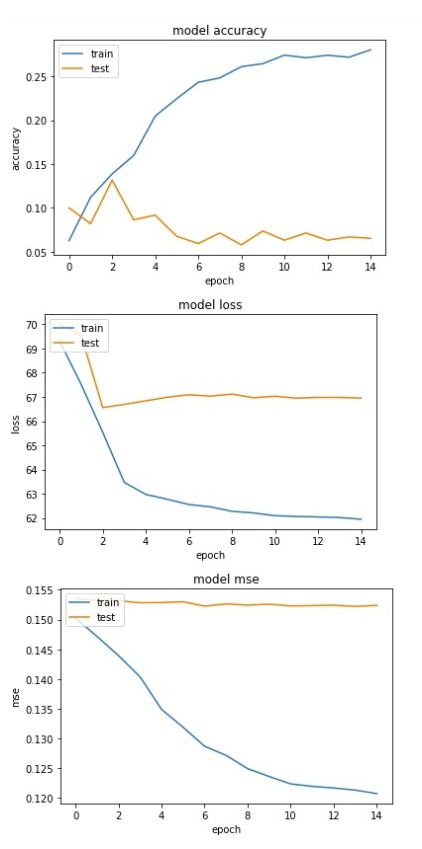
\includegraphics[width=0.05\textwidth]{images/Conf_1.PNG} & 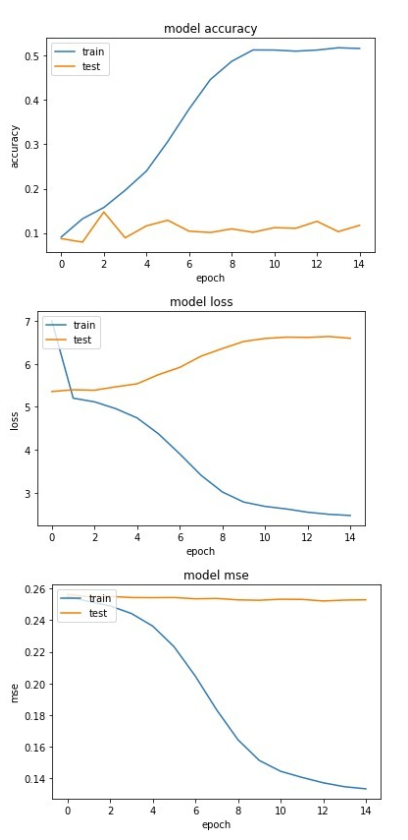
\includegraphics[width=0.05\textwidth]{images/Conf_2.PNG} &  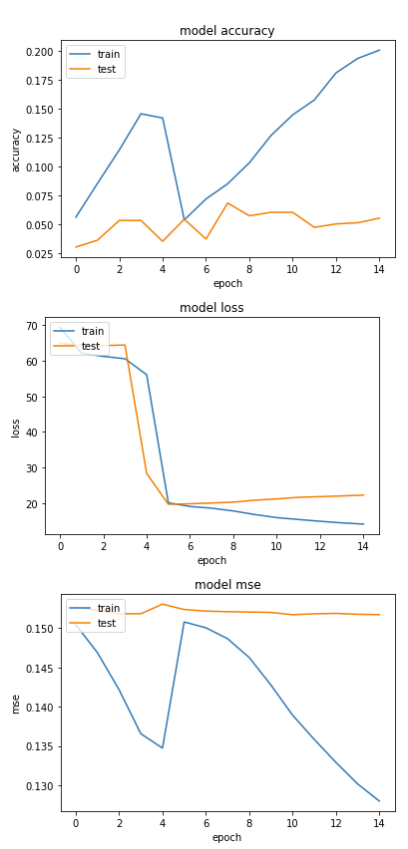
\includegraphics[width=0.05\textwidth]{images/Conf_3.PNG} & 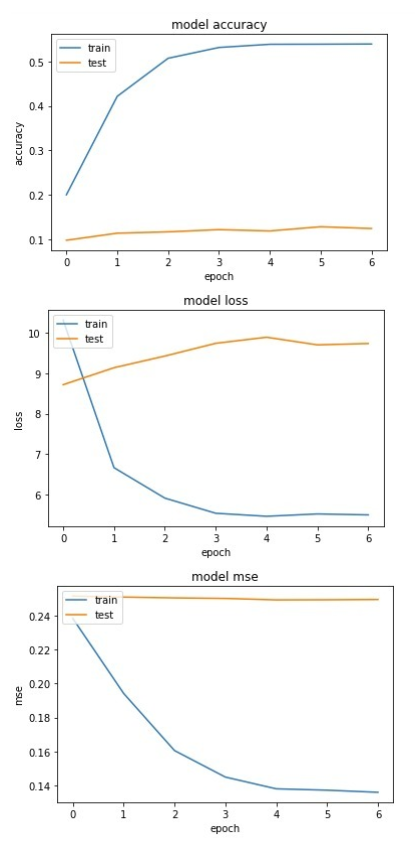
\includegraphics[width=0.05\textwidth]{images/Conf_4.PNG} \\\hline
\end{tabular}
\end{center}

\vspace{2em}

Results Conclusion:
\begin{itemize}
    \item The architecture with the custom layer over-fitted to train from the 4th epoch. It could continue working more but Google Colab disconnected so we managed to run it 15 epochs.
    \item The architecture with the dense arrived to early stopping after 6 epochs only (on train loss), meaning that there was a limit to the over-fit that it could made to the train.
    \item In every configuration we couldn't reach more then 11\% accuracy on the test and validation.
    \item We could use different probability threshold for classification of 1, and maybe get better results. It could be an idea for future research.
\end{itemize}
}

    

    \column{0.32}
    
    \block{Conclusions}{
        The proposed model is another way of utilizing the attention mechanism to create a sentence and document embeddings.
        This work is different from the previous work in the sense of three points. First, it uses the hierarchical attention that mirror the document structure. Second, it uses the structured self-attention, which creates a very good embedding. Third, the abstract features are weighted and automatically learned during the learning process taking in consideration the previously classified sentences. 
        We believe that combining the reinforcement learning with sequence to-sequence training objective is an interesting direction for further research.
            }
    
    \block{References}{
    Colab - https://colab.research.google.com/drive/1fc2GYdHcewXZRS-pU1ZDqntKKjulvFlx
    
    Original Paper - https://ieeexplore.ieee.org/stamp/stamp.jsp?arnumber=8344797
    
    \vspace{6em}
    
        \begin{tabular}{c}
            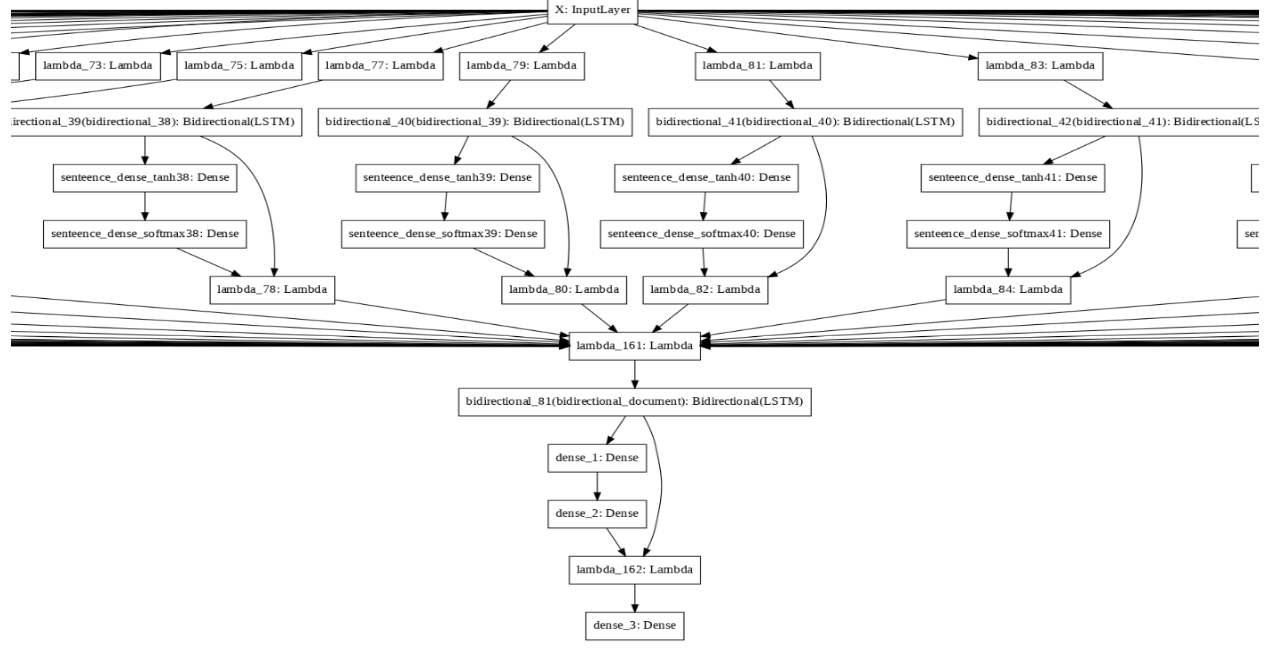
\includegraphics[scale=1.5]{Model.PNG} \\
            Figure 1: Our Model
        \end{tabular}
        
        \vspace{2em}
        
        \begin{tabular}{c c}
            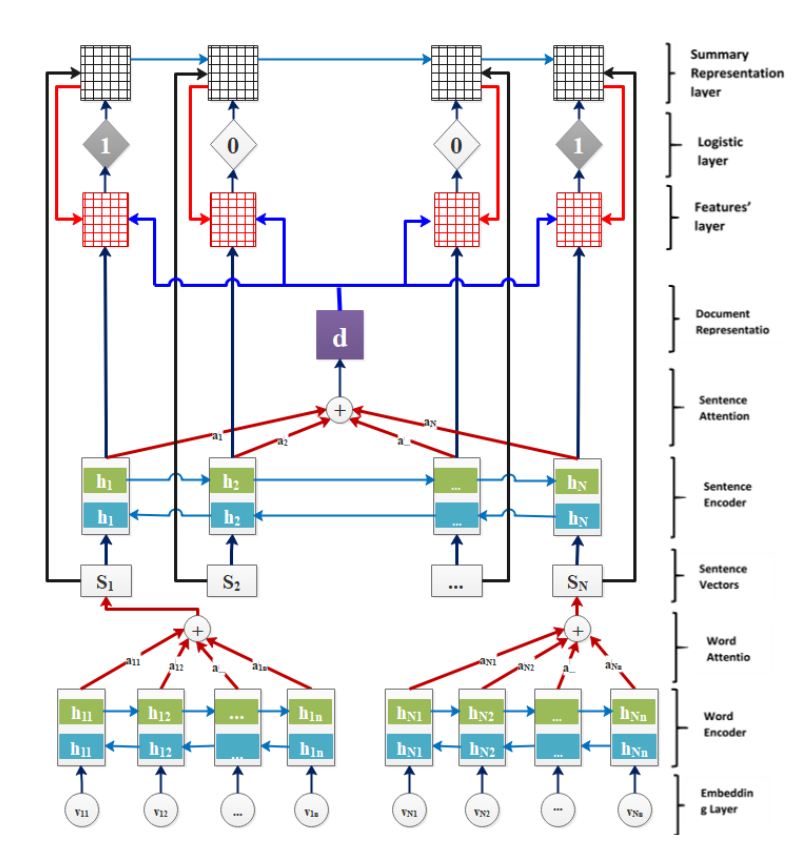
\includegraphics[scale=1.2]{images/Architecture.PNG} & 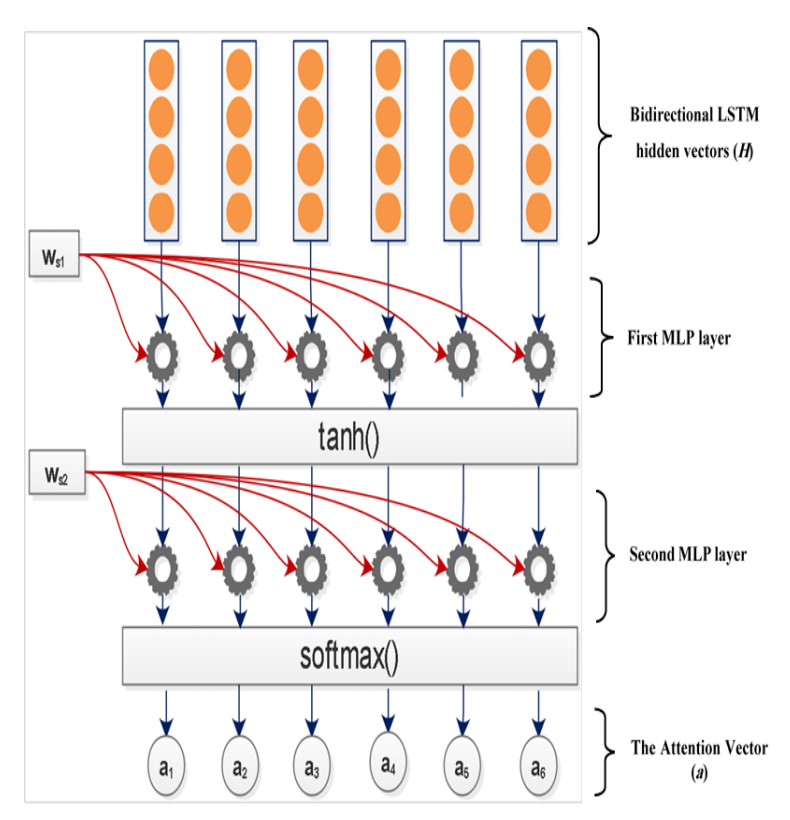
\includegraphics[scale=1.2]{images/Attention.PNG} \\
            Figure 2: Architecture & Figure 3: Attention
        \end{tabular}
    }
    

        
\end{columns}


\end{document}